\documentclass[conference]{IEEEtran}
\IEEEoverridecommandlockouts


\usepackage[T2A]{fontenc}
\usepackage[utf8]{inputenc}
\usepackage[english,russian]{babel}
\usepackage{cite}
\usepackage{amsmath,amssymb,amsfonts}
\usepackage{algorithmic}
\usepackage{graphicx}
\usepackage{textcomp}
\usepackage{xcolor}
\def\BibTeX{{\rm B\kern-.05em{\sc i\kern-.025em b}\kern-.08em
    T\kern-.1667em\lower.7ex\hbox{E}\kern-.125emX}}
\begin{document}


\title{Анализ данных с КиноПоиска}

\author{\IEEEauthorblockN{Дмитрий Курносов}
\IEEEauthorblockA{\textit{Институт прикладной математики и механики} \\
\textit{Санкт-Петербургский политехнический университет Петра Великого}\\
Санкт-Петербург, Россия \\
dima2202888@yandex.ru}
\and
\IEEEauthorblockN{Никита Лансков}
\IEEEauthorblockA{\textit{Институт прикладной математики и механики} \\
\textit{Санкт-Петербургский политехнический университет Петра Великого}\\
Санкт-Петербург, Россия \\
nl516@yandex.ru}
\and
\IEEEauthorblockN{Михаил Нахатович}
\IEEEauthorblockA{\textit{Институт прикладной математики и механики} \\
\textit{Санкт-Петербургский политехнический университет Петра Великого}\\
Санкт-Петербург, Россия \\
0000-0002-6279-1130}
\and
\IEEEauthorblockN{Максим Смольский}
\IEEEauthorblockA{\textit{Институт прикладной математики и механики} \\
\textit{Санкт-Петербургский политехнический университет Петра Великого}\\
Санкт-Петербург, Россия \\
mithridatus@mail.ru}
}

\maketitle

\begin{abstract}
Эта статья описывает процесс анализа данных с сайта кинопоиск. В рамках статьи рассмотрены процессы получения данных, хранения данных, а также последующей обработки данных для решения 
поставленных задач.
\end{abstract}

%\begin{IEEEkeywords}
%big data, data sciense
%\end{IEEEkeywords}

\section{Введение}

Индустрия фильмов развивается с каждым годом и является важной частью в жизни каждого человека. Также растёт интерес к кинопрокату, ежегодно растёт оборот денежных средств в киноиндустрии, а также качество съёмки и число людей, задействованных в процессе работы над новыми фильмами.

КиноПоиск - крупнейший русскоязычный интернет-сервис о кино. Данный сервис предоставляет информацию о различных фильмах, актёрах, новостях кино и т.д.

В данной работе представлен анализ данных о фильмах: рассмотрены взаимосвязи между 
различными характеристиками фильмов и построены распределения фильмов по различным критериям. В рамках данной работы мы делали упор на статистические методы анализа данных.

\section{Данные}

\subsection{Получение данных}

Для скачивания данных использовался сторонний API для доступа к актуальной информации КиноПоиска. Так как данный API предоставляет информацию о фильме только по его идентификатору, для получения всех идентификаторов фильмов был выполнен парсинг самого сайта КиноПоиск. Коннектор написан на языке Python с использованием пакета PyMongo для работы с MongoDB из Python. Всего было выкачено 654165 фильмов. Объём данных составил 3.4 Гб.

\subsection{Структура данных}

Выгруженную информацию о фильмах можно поделить на блоки, представленные на Рис.~\ref{fig:1}. Каждый фильм содержит некоторые общие сведения такие как название, год производства, жанры и т.д. Также есть список создателей, то есть список всех актёров, режиссёров и т.д., задействованных в создании фильма. Различные рейтинги, в число которых входит рейтинг из базы IMDb. Рецензии зрителей и бюджет фильма, в который также входят сборы.

\begin{figure}[ht!]
	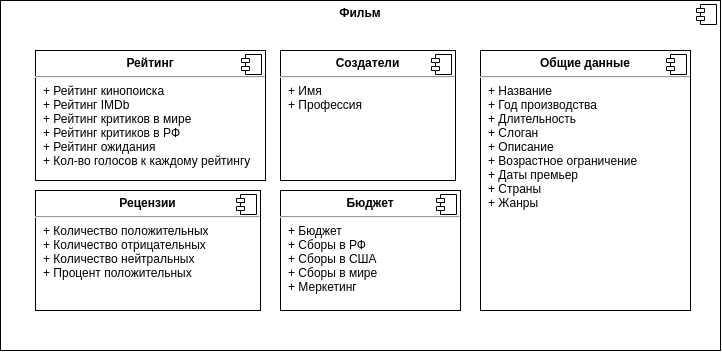
\includegraphics[width=\linewidth]{../report/images/dataStructure}
	\caption{Схема представления данных.}
	\label{fig:1}
\end{figure}

\subsection{Обработка данных}

Все вычисления производились при помощи системы распределённых вычислений - Apache Spark.


\section{Статистические задачи}
\subsection{Корреляция оценок зрителей и критиков}
\subsection{Корреляция рейтинга КиноПоиска и рейтинга IMDb}
\subsection{Распределение фильмов по странам}
\subsection{Распределение фильмов по прибыльности}
\subsection{Распределение фильмов между странами по годам}
\subsection{Распределение фильмов по возрастным ограничениям и годам}
\subsection{Средний рейтинг российских фильмов по годам}

\section{Исследовательские задачи}
\subsection{Прогноз количества фильмов по жанрам на 10 лет}

\section{Дальнейшие исследования}

\section{Заключение}

\end{document}
